% Copyright 2022 by Marek Rychly <rychly@fit.vut.cz>.
%
\documentclass[10pt,xcolor=pdflatex,dvipsnames,table,oneside]{book}
% babel and encoding
\usepackage[slovak]{babel}
\usepackage[T1]{fontenc}
\usepackage[utf8]{inputenc}

\usepackage{csquotes}% correct/formal language-specific quotations
\usepackage{microtype}% character protrusion, font expansion, adjustment of interword spacing, additional kerning, tracking, etc.
\usepackage{hyperref}% hyper-refs in PDF
\usepackage{graphicx}
\usepackage{caption}

\author{
  Marek Mudroň\\
  \texttt{xmudro04}
  \and
  Samuel Repka\\
  \texttt{xrepka07}
  \and
  Barbora Šmahlíková\\
  \texttt{xsmahl00}
}
\title{Príprava dát a ich popisná charakteristika}
\date{zima 2022}

\begin{document}

\pagenumbering{roman}

\hypersetup{pageanchor=false}% disable hyperref anchor to title page as maketitle enforce pagenumbering to arabic which colides the titlepage with the first arabic page below
\maketitle
\hypersetup{pageanchor=true}
\tableofcontents

\newpage% force page-break to start the page numbering on a new page
\pagenumbering{arabic}


\chapter{Dátová sada}

V tomto projekte sa zaoberáme exploráciou, čistením a tvorbou popisnej charakteristiky pre open-source dátovú sadu 
\textit{Palmer Archipelago (Antarctica) penguin data}. Ide o dátovú sadu, ktorej obsahom sú informácie o fyziologických a demografických vlastnostiach troch druhov tučniakov. Dataset obsahuje súbory \texttt{penguins\_lter.csv} a \texttt{penguins\_size.csv}. Oba obsahujú informácie k rovnakým jedincom,  no \texttt{penguins\_lter.csv} poskytuje okrem informácií obsiahnutých v \texttt{penguins\_size.csv} aj dáta k hodnotám stabilných izotopov uhlíka  ($\delta^{13}$C)  a dusíka  ($\delta^{15}$N)  v tele. Tieto údaje sa používajú už od roku 1980  poskytujú hodnotné informácie k životospráve a migračným vzorcom tučniakov. Preto pre naše účely využívame informácie obsiahnuté v \texttt{penguins\_lter.csv}.

\chapter{Exploratívna analýza}

Prvým z atribútov, ktorý sa medzi jednotlivými položkami datasetu nelíši je \texttt{studyName}, ten obsahuje pre každého jedince rovnakú hodnotu \textit{PAL0708}.

Dataset obsahuje v atribúte \texttt{Species} názov jedného z troch druhov  tučniakov
\begin{enumerate}
  \item Adelie Penguin (Pygoscelis adeliae)
  \item Chinstrap penguin (Pygoscelis antarctica)
  \item Gentoo penguin (Pygoscelis papua)
\end{enumerate}

\begin{figure}[h]
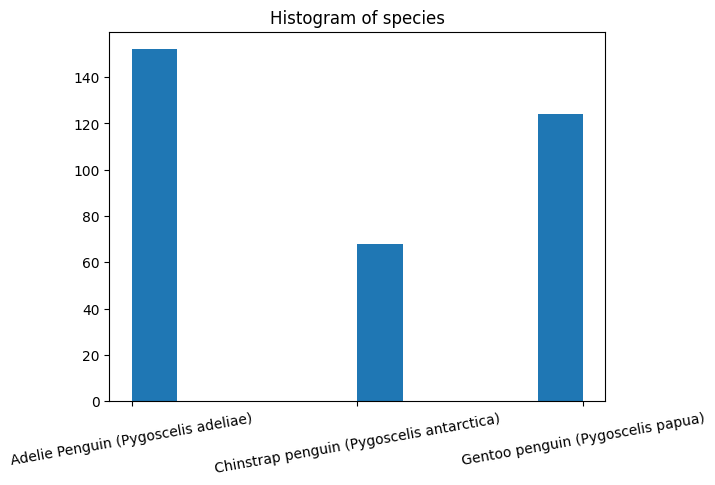
\includegraphics[width=10cm]{img/species.png}
\centering
\end{figure}
\pagebreak





Podľa datasetu, každý druh obýva niektoré z nižšie uvedených ostrovov. Demografické rozloženie sa medzi druhmi líši. Informácia je obsiahnutá v atribúte \texttt{Island}.
\begin{enumerate}
  \item Torgersen
  \item Biscoe
  \item Dream
\end{enumerate}

\begin{figure}[h]
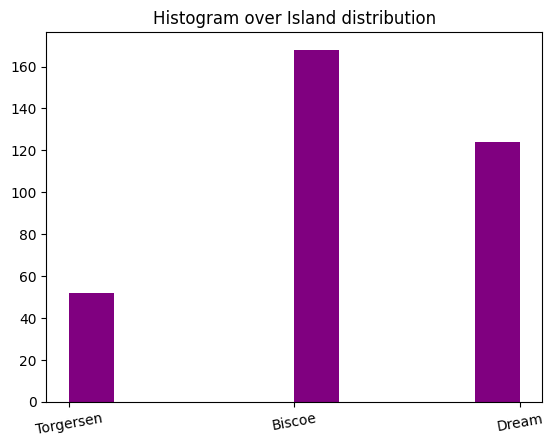
\includegraphics[width=8cm]{img/island.png}
\centering
\end{figure}



V atribúte \texttt{Region} je uvedená oblasť výskytu daného jedinca. Táto je pre každého z nich rovnaká a obsahuje hodnotu \textit{Anvers}.

Atribútom \texttt{Stage} uvádza pre každého jedinca rovnakú hodnotu \textit{Adult,~1~Egg~Stage}. Identifikátor každého z jedincov je v atribúte \texttt{Individual~ID}.

\texttt{Clutch Completion} obsahuje informáciu o tom, či bol jedince pozorovaný s hniezdom obsahujúcim viac ako 2 vajíčka. \texttt{Date Egg} uvádza dátum, kedy bol záznam k danému jedincovi vytvorený.

Atribúty \texttt{Culmen Length (mm)} a  \texttt{Culmen Depth (mm)} poskytujú rozmery zobáku. Jeho   výšku a dĺžku v milimetroch, v tomto poradí.
Dĺžka krídel tučniaka je obsiahnutá vo \texttt{Flipper Length (mm)} a taktiež je v milimetroch. Telesnú hmotnosť v gramoch poskytuje atribút \texttt{Body Mass (g)}.



\newpage
Pohlavie je uvedené v atribúte \texttt{Sex}. Vidíme, že jedna z položiek tohto atribútu obsahuje nevalidnú hodnotu '.'.

\begin{figure}[t]
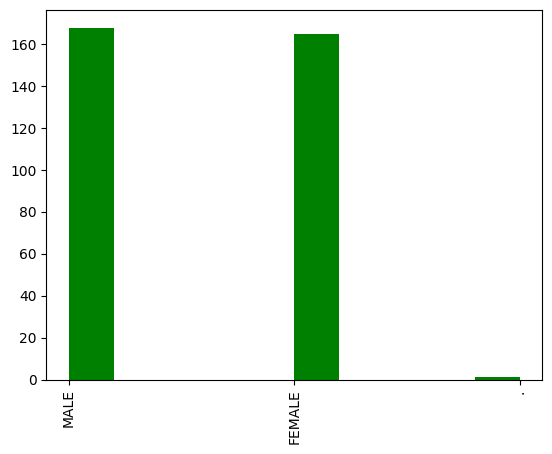
\includegraphics[width=8cm]{img/the_thing.png}
\centering
\end{figure}

Ďalšími z relevantných atribútov sú už spomínané ($\delta^{13}$C) a ($\delta^{15}$N) uvedené v atribútoch \texttt{Delta 13 C (o/oo)} a \texttt{Delta 15 N (o/oo)}.
% Samo, viac nemam sajnu co by som ti tu este mohol dopisat tak to necham na teba :)

\chapter{Príprava dátovej sady pre dolovacie algoritmy}
% Barbora s tymto ti nepomozem :)


\end{document}